\section{Motivation: social network models}
Is it possible to build a parsimonious mathematical model that captures the 
behavioral tendencies of individuals in how they form relationships?\\  % in a group?

This is the question that led us to study parameter estimation methods for exponential 
families, with a particular interest in models used to describe social network data.  
Formally, a \emph{social network} is the collection of \emph{actors} and the 
\emph{relations}, or \emph{ties}, between each pair of actors.
Social scientists have studied social networks as a discipline since as early as the 
1930s when Jacob L. Moreno introduced the sociogram, a diagram that corresponds to
the mathematical graph with individuals in a group 
represented by nodes and the presence of a relation between 
individuals by an edge \citep[Chapter 3]{Wasserman:1994}.  
A sociogram depicting the marriage network data among sixteen 
important families in Renaissance Florence \citep{Padgett} is depicted in 
Figure~\ref{F:Florentine} and another depicting the affinity, or ``liking" relation, among 18 
monks in a monastery in New England in the late 1960s \citep{Sampson} is depicted in 
Figure~\ref{F:Sampson}.  In such settings, a social scientist is often interested in 
understanding whether relations arise out of friendliness or a strategy for alliance 
building, that is, driven by actor-specific attributes or by the structure of  the relations themselves.
\begin{figure}[h!]
\begin{center}
\includegraphics[width=5in]{florentine} %,keepaspectratio
\end{center}
\caption[\citeauthor{Padgett}'s \citeyearpar{Padgett} Florentine marriage network]{
\citeauthor{Padgett}'s \citeyearpar{Padgett} Florentine marriage network.  \citeauthor{Padgett} recorded the marriage network among 16 Florentine families around 1430.  At the time, two factions, one revolving around the 
Medicis and the other around the Strozzis, vied for political control of the city.   
Data is available through and plotted using the \texttt{ergm} package \citep*{ergm:R} in 
R \citep*{R}.}
\label{F:Florentine}
\end{figure}

\begin{figure}[h!]
\begin{center}
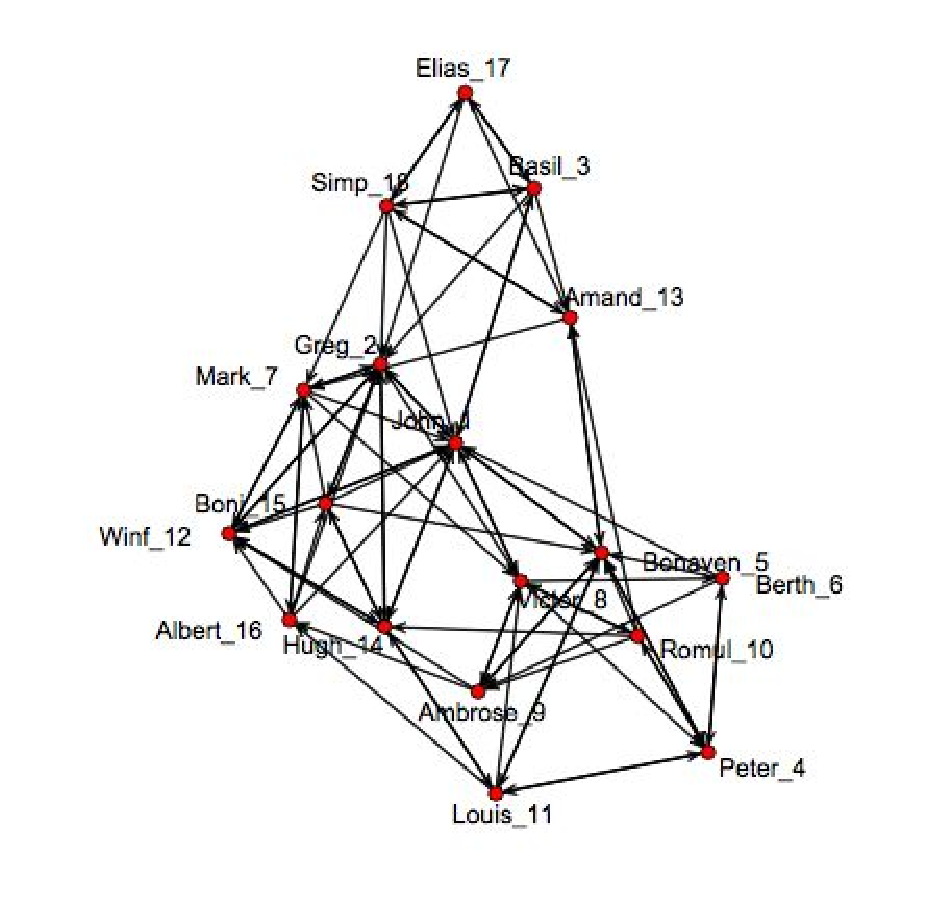
\includegraphics[width=5in, trim=0.2in 1in 0.3in .6in, clip=true ]{samplike} % l b r t
\end{center}
\caption[\citeauthor{Sampson}'s \citeyearpar{Sampson} monastery affinity network]
{\citeauthor{Sampson}'s \citeyearpar{Sampson} monastery affinity network.  \citeauthor{Sampson} collected data to define a ``liking" network among 18 monks 
in a New England monastery in the late 1960s.  Since ``liking" is a directional 
relation, the presence of a relation is depicted by an arrow rather than a line.  Data 
is available through and plotted using the \texttt{ergm} package \citep{ergm:R} in R.}
\label{F:Sampson}
\end{figure}

Stochastic network models were developed as early as 1959 in the seminal works of 
\citet{Gilbert} and \citet{Erdos}, resulting in a simple probabilistic model that is 
now referred to as the Bernoulli model or the Erd\"{o}s-R\'{e}nyi-Gilbert model.  Over 
the last forty years, more sophisticated stochastic network models have flourished;  
notable landmarks include the $p_1$ model of \citet{Holland:1981} which captures the 
reciprocal tendency of relationships in directed networks, and the $p^*$ model of 
\citet{Frank:1986} which describes the transitive tendency of relationships in 
undirected networks.  These models laid the foundation for the more general 
\emph{exponential random graph models (ERGM)}, a class of exponential family 
models that are now routinely used to model network data and are presented in 
detail in Section~\ref{S:ERGM examples}.\footnote{To be precise, they should
be called ``exponential \emph{family} random graph models", but apparently
this is too cumbersome.} 
% \citep{logit,Pattison:1999,Handcock:2006,introp*,advancesp*,recentp*,ergm,Morris:
%2008,Goodreau:2009,Goldenberg:2009}.

%\subsection{THE ISSUE -- DEPENDENCE}
At their core, stochastic network models attempt to describe whether or not a tie 
forms between each pair of actors in a group.
%  In the Florentine marriage network depicted in Figure~\ref{Padgett}, a model fit  
It has long been observed that relations, especially those involving humans, do not 
form in isolation; rather, they form in an interdependent manner.  Whether or not a 
relation forms between individuals $A$ and $B$ may very well depend on whether or not 
relations form between $B$ and $C$ and $C$ and $A$.  This has profound implications 
for the social scientist, necessitating a new ``network" perspective that recognizes 
the relational structures, such as a triangle of relations between actors $A$, $B$, 
and $C$, as factors in the analysis \citep[Chapter 1]{Wasserman:1994}.  This perspective has 
garnered increasing attention across different social and behavioral science 
disciplines over the last forty years, as evidenced by the rapid growth in publication 
of social network related papers \citep[Chapter 1]{Knoke:2008}.
% in the social science literature 
  
For the statistician, the network perspective means that the model should not break the 
network down into independent components, each containing two actors.
Instead, a good model will consider important relational structures in the observed network 
and clarify their contribution in shaping the global outcome.   
Accompanying the model must also be a computational algorithm to calibrate the model 
parameters to the network data.  
%In fact, this is the focus of our research.
In fact, writing down the expression for an uncalibrated ERGM turns out to be quite
straightforward; it is fitting the model
to data that is an open research problem and the focus of this dissertation.

Typically, parameter estimation for statistical models is done through the method of 
\emph{maximum likelihood} in which values for the parameters called \emph{maximum 
likelihood estimators (MLE)} that index the model to make the observed data most likely 
are calculated.
Many methodologies have been developed over the years to address the difficulties
in this process for exponential families
including Besag's \emph{pseudolikelihood} approach \citep{Besag:1974,Strauss:1990}, 
\citeauthor{Geyer:1992}'s \citeyearpar{Geyer:1992}
\emph{Markov chain Monte Carlo Maximum Likelihood} (MCMC-ML) approach, and 
\emph{stochastic approximation}.\footnote{Stochastic approximation has more general
applications in root finding, but is frequently used for parameter estimation.}
In fact, it was the absence of usable methodologies in parameter estimation that 
restricted earlier models like $p_1$ and $p^*$ to their simpler modeling capabilities.

%the simple expression belies the difficulties involved in fitting the model to data.
%In this paper, we describe further advances to these methodologies that address some of the
%pathologies researchers have encountered with these approaches.

Once model parameters are properly estimated, the completed model can be used to simulate 
new random networks whose distribution retains essential characteristics of 
the observed network.  Researchers can then use this 
to further test hypotheses about the process of relationship formation.  
In this dissertation, we consider the ability to do statistical inference 
as the end goal of parameter estimation rather than the parameter values 
themselves.  This requires obtaining the maximum likelihood \emph{distribution} which
can then be used to construct confidence intervals and evaluate hypotheses.

%Similarly, exponential random graph models have a deceptively simple form \eqref
%{E:ERGM} that belies the challenges involved in estimating the model parameters.  

%Network researchers have developed many descriptive statistics to capture 
%characteristics of a network.  For example, the number of ties going to a particular 
%actor is one measure of that actor's prestige in that network \citep{Wasserman:1994}.  

Finally, it should be noted that although problems from the social sciences provide much of the 
motivation for social network analysis and our research here, network models can in 
fact be applied to problems in a broad range of disciplines including political 
science, biology, epidemiology, and computer science and may be of interest
to business practitioners in utilities or transportation.  
Actors often represent individuals but 
they may also represent entities like nation-states, protein molecules, airports, 
computers, or corporations.  The relation that connects actors 
is often friendship or actor $A$ 
``liking'' actor $B$, as in Sampson's monk data depicted in Figure~\ref{F:Sampson}, 
but the relation can be any kind, such as a business transaction or the 
Internet connectedness between computers.  Figure~\ref{F:ecoli} depicts the 
\textit{Escherichia Coli} transcriptional regulation network among 423 operons of
\citet*{Shen-Orr} based on the RegulonDB data of \citet*{Salgado}. These were 
modeled with ERGMs by \citet*{Saul:2007} and later by \citet*{Hummel}.

\begin{figure}[h!]
\begin{center}
\includegraphics[width=5in, trim=0.2in 0.in 0.2in .in, clip=true ]{ecoli} % l b r t
\end{center}
\caption[\textit{E. Coli} transcriptional regulation network of \citet{Shen-Orr}]{\textit{E. Coli} transcriptional regulation network of \citet{Shen-Orr}.  Each node is an operon and a directed edge from one node to another indicates 
that the first encodes the transcription factor that regulates the second.
Data is available through and plotted using the \texttt{ergm} package \citep{ergm:R} in R.}
\label{F:ecoli}
\end{figure}



%%%%%%%%%%%%%%%%%%%%%%%%%%%%%%%%%%%
\subsection{Why model networks?}
Before we step into a lengthy of discussion of how we model network data, it is 
worth reflecting upon the question of why network models are desirable or interesting.  We 
have already given one answer to this question in the context of the social scientist 
trying to differentiate between competing underlying forces that can shape the global 
structure of relationships: a network model will allow the researcher to 
identify if one or more actor specific variables and network structures 
contribute to the characteristic of the overall network.  That is, a good statistical 
model can see past noise in the data to
provide clarity of the underlying forces that shape the structure of an observed network
\citep*{Goodreau:2009}.   

In the context of epidemiology, a model for  
a \emph{contact network}, which is a network of the potential disease-causing ties between individuals, may be useful in understanding the general mechanism by which an epidemic can spread.  This may in turn help formulate an intervention strategy \citep*{Welch:2011}.
In computational biology, network models may be used to better understand the processes
by which proteins interact \citep*{Goldenberg:2009}.  
Some other applications of networks are the links between sites on the Internet
or the international relations between countries.  At its essence, 
a network is a conduit for flow, whether it be the flow of diseases, commodities, 
data, capital, or ideas, and network models can help us
 understand the mechanism of this flow \citep*{Kolaczyk:slides}.

\section{Exponential random graph model setup} \label{S:ERGM setup}
Networks can be modeled as a random  $n \times n$ matrix $Y$, where $n$ is 
the number of actors.
Each entry $Y_{ij}$ in the random matrix $Y$ is itself a random variable representing 
a relation from actor $i$ to actor $j$, such that:
\[
	Y_{ij} = 
	\begin{cases}
		1 & \text{if a relation exists \textit{from} actor $i$ \textit{to} actor 
$j$ (notation: $i \to j$)}\\
		0 & \text{otherwise}
	\end{cases}
	\
\]
where $i$ and $j$ take values in $1, \ldots, n$, $i \neq j$.  
Note that $Y_{ij}$ take only values of $0$ or $1$, reflecting our restriction 
on networks to those with \emph{dichotomous} relations, that is, the relation between a pair 
of actors is either present or absent.  In addition, we do not allow  
$i \to i$ and always have $Y_{ii} = 0$.  In the special case that 
$Y_{ij} = Y_{ji}$ and thus the matrix $Y$ is symmetric, the network is referred to as an
\textit{undirected} network or graph, such as in the case of the Florentine marriage 
network depicted in Figure~\ref{F:Florentine}.  A network is \textit{directed} if it is 
not undirected, as in the case of monastery affinity network depicted in 
Figure~\ref{F:Sampson}.  

The exponential family random graph model (ERGM) commonly used in the network 
literature for $Y$ has probability mass function of the following form:
\begin{align}
	f_\eta(y) = P_{\eta}(Y=y) = \frac{1}{ \kappa( \eta) } e^{ \inner{ \eta, g(y)}  } \qquad y \in \YY, \label{E:ERGM}
\end{align}
where $g(y)$ is a $d$-vector of statistics, $\eta$ is a $d$-vector of parameters, 
$\inner{\fatdot,\fatdot}$ denotes the bilinear form
\begin{align*}
	\inner{ \eta, g } = \sum_{i=1}^d g_i \eta_i,
\end{align*}
and $\YY$ is the sample space of all possible networks.
So that \eqref{E:ERGM} integrates to 1, $\kappa(\eta)$ is a normalizing constant such that
\begin{align}
   \kappa(\eta) &= \int e^{ \inner{ \eta, g(x)}  } \, d \mu(x) \label{E:kappa}
\end{align}
where $\mu$ is a measure on $\YY$.  In fact, \eqref{E:ERGM} is exactly the form of 
an exponential family distribution in \emph{canonical form} \citep[Chapter 1.4]{tpe}.  The only distinction that makes this an ERGM is that $\YY$ is specified to be the 
discrete state space of all possible network configurations.

We rely on many properties of exponential families.  Define 
\begin{align}
   \Xi &= \{ \eta \in \RR^d : \kappa(\eta) < \infty \}.  \label{E:paramspace}
\end{align}
An exponential family is \emph{full} if the natural parameter  space is 
\eqref{E:paramspace}, and \emph{regular} if, in in addition, $\Xi$ is an open set.
%The exponential family is \emph{full} if the natural parameter space is \eqref
%{E:fullparam}, and \emph{regular} if, in 
%addition, $\Xi$ is an open set.  
We say an exponential family is \emph{minimal} if the natural statistic and 
natural parameter are not each concentrated on a hyperplane. 
Minimality guarantees that if an MLE, denoted $\etaMLE$, exists, 
it is unique \citep{Geyer:gdor}.


Define the \emph{cumulant} function as $c(\eta) = \log \kappa(\eta)$ and
denote the observed data as $\yobs$.  We can then express 
the log likelihood of \eqref{E:ERGM} as
\begin{align}
	\ell( \eta ) = \inner{ \eta, g(\yobs)} - c( \eta). \label{E:loglike}
\end{align}

The appeal of exponential families in the setting of complex dependence phenomena such 
as networks stems from their simplicity and maximum entropy property 
\citep{Jaynes:1978,Geyer:1992}.
By choosing statistics of interest on the data, one fully specifies a model that gives 
the 
most reasonable inference possible derived solely from those statistics.  
Furthermore, exponential families have been 
well-studied \citep{Barndorff,Brown:1986} and utilized over the decades and have 
desirable properties such as the MLE uniqueness noted above.

%%%%%%%%% NETWORK STATISTICS
Ideally then, a network researcher need only specify relational structures of 
interest to define an ERGM.  
\citet*{Wasserman:1996, Pattison:1999, logit, introp*} describe many of 
the classical network statistics that one might include in the natural statistics vector 
$g(y)$.  In these works, the researchers' primary 
consideration in defining a network statistic is a relational structure's 
scientific interpretability.  
For example, in a directed affinity network, a sociologist may be 
interested in the propensity for individuals to form \emph{reciprocal} relations, where 
ties exist $i \to j$ and $j \to i$, or \emph{transitive} relations, where 
ties exist $i \to j$, $j \to k$, $i \to k$.  The statistics vector $g(y)$ 
that captures these can be defined by
\begin{align*}
	g(y) = \left ( \sum_{i<j} Y_{ij}Y_{ji}, \sum_{i \neq j \neq k} Y_{ij}Y_{jk}Y_{ik} 
			\right )  
\end{align*}
where its components count the number of reciprocal and transitive relational 
structures.  
Such a model, with parameters appropriately calibrated to the affinity network, 
should then generate networks that exhibit a frequency of reciprocal and 
transitive relations similar to that of the observed data.
We will not discuss the merits of all the different network statistics 
here; in fact, there is essentially an unlimited number of potential network statistics.
What is important is that these statistics can be transparently calculated for a 
given network and the inclusion of them in $g(y)$, paired with their parameter 
components in $\eta$, allows the model \eqref{E:ERGM} to calculate probabilities of 
different global network outcomes $y$.  \citet*{ergm:userterms} 
go so far as to provide an interface for one to
customize and create her own network statistic of interest and model it in the 
\texttt{ergm} package in R.

%%%%%% RECENT NETWORK STATISTICS
More recently, \citet*{Handcock:2006, Hunter:2006, recentp*} developed
new network statistics with particular emphasis on the sensibleness of 
the distributions generated from the specified models.  
These came about in response to the repeated discovery that poorly behaving models can
result when a researcher only considers the scientific significance of network
statistics before including them in a model.
To be fair, it is not 
at all obvious from their definitions which network structures might work poorly
together in an ERGM.  A fairly complete description of these more recent network 
statistics is in \citet*{Morris:2008}.  
%We return to this issue in more detail in Section~\ref{S:Non-existent MLE}.
%In addition, the issue of model selection between competing models has not been 
%addressed though \citet{GOF} have begun making strides in this area.  Both of these 
%areas are active area of research.



%%%%%%%%%%%%%%%%%%%%%%%%%%%%%%%%%%%
\subsection{Intractable normalizing constant} \label{S:intractable}
We now return to the issue of why parameter estimation for ERGMs and 
similar exponential family models on discrete state spaces can be challenging.
Despite the tremendous appeal of the exponential family framework, one 
immediate and sizable problem is that the summation in \eqref{E:kappa} for the 
normalizing constant $\kappa(\eta)$ is over all possible 
networks in the sample space $\YY$ and can be prohibitively expensive to 
evaluate for networks of even moderate size.
For an undirected network with $n$ actors, there are $2^{{n\choose 2} }$ 
different possible networks in $\YY$.  Table~\ref{T:number graphs} shows how rapidly this number grows; 
unless dealing with networks of 9 actors or less, the likelihood function 
should not be directly evaluated.  See Appendix~\ref{A:Triangle count}
for our approach for counting simple network statistics in the 9-node network
relying on numerous tricks in data representation and computation.

\begin{table}[h!] 
\caption{Sample space size for undirected networks with different number of 
actors.}

\begin{tabular}{ccl} 
\hline 
Nodes & Possible Edges & Total Graphs \\ [1ex]
\hline
5 & ${5 \choose 2} = 10$ & $2^{10} = 1024$ \\ [1ex]
6 & ${6 \choose 2} = 15$ & $2^{15} = 32,768$ \\ [1ex]
7 & ${7 \choose 2} = 21$ & $2^{21} = 2,097,152$ \\ [1ex]
8 & ${8 \choose 2} = 28$ & $2^{28} = 268,435,456$ \\ [1ex]
9 & ${9 \choose 2} = 36$ & $2^{36} = 68,719,476,736$ \\ [1ex]
10 & ${10 \choose 2} = 45$ & $2^{45} = 3.518437\times10^{13}$ \\ [1ex]
\hline 
\end{tabular} \label{T:number graphs}
\end{table}

%%%%%%%%%%%%%%%%%%%%%%%%%%%%%%%%%%%
\subsection{Covariate data} \label{S:Covariate}
Information about a particular actor, say gender, can be incorporated as 
covariate data into the model with little difficulty.
Often, a social scientist looks to include such information because she is interested in
whether or not there is an \emph{assortative mixing} effect, that is, whether individuals of the same ``type" tend to make more relations with others of that type \citep{Goodreau:2009}.  
Suppose we wish to incorporate $p$ such exogenous attributes for our $n$-actor network.  
This information can be represented by an $n \times n \times p$ matrix $X$, whose 
$ijk$th element is the value of the $k$th attribute in the potential relation from actor
$i$ to $j$ \citep*{Fienberg:1981,ergm}.  We include such factors in our model 
of an adolescent friendship data set in Section~\ref{S:Example:FauxMagnolia}.

Like the other network statistics discussed, the statistics that comprise $X$ can 
be transparently calculated from data and hence included in the canonical 
statistics vector as $g(y, X)$,
with the canonical parameter vector $\eta$ lengthened accordingly.
The parameter estimation methodology is unchanged from before (so long as $p$ is not
excessively large), and while this greatly expands the
usefulness of ERGMs to the researcher, there are no new issues for us to consider
from a statistical modeling perspective.
Thus we will continue to use $g(y)$ instead of $g(y,X)$ for simplicity.  



%%%%%%%%%%%%%%%%%%%%%%%%%%%%%%%%%%%
\section{Examples of ERGMs} \label{S:ERGM examples}
We now review the classical Erd\H{o}s-R\'{e}nyi-Gilbert, $p_1$, and $p^*$ models to give both a sense of commonly used network structures as well as parameter estimation methodologies.

\subsection{Erd\H{o}s-R\'{e}nyi-Gilbert model} \label{S:Erdos}
The simplest example of an exponential random graph is the Erd\H{o}s-R\'{e}nyi-Gilbert 
model \citep{Erdos,Gilbert}, also referred to as a Bernoulli network model, which 
assumes that each actor forms a relation to every other actor independently with the 
same probability $p$ \citep{ergm}.  The ERGM can be expressed as
\begin{align*}
	P_{\eta}(Y=y) &= \frac{1}{\kappa( \eta) }e^{\eta g(y)}  \qquad y \in \YY, 
\end{align*}
where the only network statistic is a count of the number of edges for the directed network
\begin{align*}
%	g(y) = \frac{1}{N}\sum_{i \neq j} y_{ij},
	g(y) = \sum_{i \neq j} y_{ij}
\end{align*}
and the probability of a tie formation between any pair of actors is the constant
\begin{align*}
	p = \frac{e^{\eta}}{1+e^{\eta}}.
\end{align*}
%and thus the $Y_{ij}$ are mutually independent of one another.  
The MLE of $\eta$, $\etaMLE$, can be found analytically to be the logit of the 
fraction of ties that are present in the observed data set, 
\begin{align*}
	\etaMLE = \logit \left ( \frac{\sum_{i \neq j} y_{\textrm{obs}, ij}}{ N } \right )
\end{align*}
where $N = n(n-1)$, the number of possible ties in a directed network with $n$ actors.  
The MLE 
for $\eta$ is thus easily calculated from the observed data. The independence 
assumption, however, is too unrealistic for all but the simplest of cases; usually, 
a researcher is interested in modeling different probabilities of tie formations 
between actors.  Thus the Erd\H{o}s-R\'{e}nyi-Gilbert model may be most 
useful as a ``null'' model, though it is arguably too simple even for this.

%%%%%%%%%%%%%%%%%%%%%%%%%%%%%%%%%%%
\subsection{The $p_1$ Model} \label{S:p1}
\citet{Holland:1981} made advances in relaxing this independence assumption  with 
their $p_1$ model.  They focused on two empirical observations from sociometric 
studies:
\begin{itemize}
\item Reciprocation: there tend to be a ``surplus" of mutual relationships in network 
data sets compared to a uniform distribution of directed relationships.
\item Stars: some individuals attract a surplus of choices compared to a uniform 
distribution of directed relationships.
\end{itemize}
\citeauthor{Holland:1981} then constructed a family of distributions with parameters 
to control the probability of observing different numbers of mutual relationships and 
stars.  
Focusing on the \textit{dyad}, the set of a pair of actors and the possible relations 
between them, as the basic building block, they proposed the following model:
\[
	P( Y = y ) = \frac{1}{ K( \rho, \theta, \{ \alpha_i \}, \{\beta_j \} )}\exp \left 
\{  \rho m(y) + \theta y_{++} + \sum_i \alpha_i y_{i+} +  \sum_j \beta_j y_{+j}\right 
\}
\]
subject to $\sum_i \alpha_i = \sum_j \beta_j = 0$, where
\begin{align*}
	\rho &= \text{``force of reciprocation" or mutuality parameter}\\
	m(y) &= \sum_{i \neq j} y_{ij}y_{ji}, \quad \text{number of mutual relationships 
in $y$}\\
	\theta &= \text{``density" or overall choice effect parameter}\\
	y_{++} &= \sum_{i \neq j} y_{ij}, \quad  \text{total number of relations in $y$}\\
	\alpha_i &= \text{``productivity" or ``expansiveness" effect parameter for node $i
$}\\
	y_{i+} &= \sum_{j} y_{ij}, \quad  \text{``out-degree" for node $i$ in $y$}\\
	\beta_j &= \text{``attractiveness" or ``popularity" effect parameter for node $j$} 
\\
	y_{+j} &= \sum_{i} y_{ij}, \quad  \text{``in-degree" for node $j$ in $y$}\\
	K &= \text{normalizing constant}
\end{align*}

By defining new dyad random variables, $D_{ij} = (Y_{ij}, Y_{ji} )$, \citeauthor
{Holland:1981}  showed that with some algebraic manipulation, the form of the model above 
can be viewed as a log-linear model with independent dyad random variables, 
$D_{ij}$.  This makes it possible to use a standard logistic regression to calculate MLEs of the parameters.

The statistical independence at the dyad level, however, means that this model will 
not capture triangular tie configurations (or anything more complicated) in which dyads are dependent.  Also, to 
reduce the number of parameters, the model assumes $\rho_{ij} = \rho$ and $\theta_{ij} = \theta$, meaning that the 
tendency towards reciprocity and forming relations is assumed to be the same across all actors.  This example 
illustrates how the parameter estimation methodology limits the scope of the model and 
what types of behavior it can capture.  

%%%%%%%%%%%%%%%%%%%%%%%%%%%%%%%%%%%
\subsection{Markov graph model}
\citet{Frank:1986} relaxed the independence assumption further with the implementation 
of \textit{Markov dependence} in which two dyads are independent, conditional on the 
rest of the graph, when they do not share a node.  The model uses only three 
configurations in an undirected network, expressed as:
\[
	P( Y = y ) = \frac{1}{K( \theta, \sigma, \tau)}\exp 
				\left \{ \theta L + \sigma S + \tau T	\right \} 
	\]
where
\begin{align*}
	\theta &= 		\text{Edge parameter} \\
	L &= 		\text{Number of edges} \\
	\sigma &= \text{2-Star parameter, propensity for individuals to have connections 
with two actors} \\
	S &= \text{Number of 2-stars ($i \leftrightarrow j$, $i \leftrightarrow k$) }\\
	\tau	&= \text{Triangle parameter, represents clustering} \\
	T &= \text{Number of triangles ($i \leftrightarrow j$, $j \leftrightarrow k$, $i 
\leftrightarrow k$)}
\end{align*}
None of the above parameters have subscript indices, reflecting the simplification 
from a \textit{homogeneity} assumption where parameters are equated if the 
network structures are the same ignoring the labels on the nodes (also called \textit
{isomorphic} configurations.  In fact, this is the same simplification \citeauthor{Holland:1981} employ for the $\rho$ and $\theta$ parameters in their $p_1$ model).

The model is the first to break dyad independence, made possible by \citeauthor{Frank:1986}' methods of parameter estimation.  In particular, \citeauthor{Frank:1986} ran
Markov chain Monte Carlo simulations of the model at multiple values for a parameter 
to determine which fit the data best.  The authors also obtained 
\emph{maximum pseudolikelihood estimators (MPLE)} from a standard logistic 
regression (we discuss the pseudolikelihood approach in Section~\ref{S:pseudolikelihood}) 
and observed that the MPLEs are close to those they arrived at from their rigorous simulations.   \citeauthor{Frank:1986} seem to conclude that MPLEs are generally quite acceptable.  


%%%%%%%%%%%%%%%%% SECTION %%%%%%%%%%%
\section{ERGM parameter estimation}
Exponential random graph models have a deceptively simple form \eqref
{E:ERGM} that belies the challenges involved in model parameter estimation.
As discussed in Section~\ref{S:intractable}, the difficulties
arise from a normalizing constant \eqref{E:kappa} which may involve 
a summation over an astronomical number of terms.
%resulting from the computationally infeasible normalizing constant \eqref{E:kappa}.  
In this section, we discuss commonly used parameter estimation methods
used for exponential families with complex dependence like ERGMs.  All approaches avoid evaluating the likelihood function directly but have properties that we
find undesirable.  
%These provide the backdrop for the new algorithm we propose in this paper.

%However, even with increasingly sophisticated simulation methods, finding MLEs for 
%ERGMs can be problematic in two ways:
%\begin{enumerate}
%\item The methodology used to find MLEs fails due to a shortcoming in the methodology 
%itself.  That is, an alternative approach might yield parameter estimates resulting in 
%a perfectly good model.
%
%\item The model itself is specified in such a manner so that it can be classified as 
%\emph{degenerate}, a term first applied to ERGMs by \citet{Handcock:Degeneracy} and 
%further clarified by \citet{Rinaldo:2009} to refer to instances where
%\begin{enumerate}
%\item Random graphs generated from the fitted model lack variability, often only 
%giving rise to unrealistic graphs, usually empty or complete (or nearly complete).
%\item the MLE does not exist.
%\item The fitted model makes the observed network highly unlikely.
%\end{enumerate}
%\end{enumerate}
%The two issues are related; for example, if the MLE does not actually exist, then 
%commonly used algorithms sent to find it will surely fail, or worse, return values 
%that the user may then treat as correct.   The issue is significant enough to be a 
%barrier to the use of ERGMs \citep{advancesp*}.



\subsection{Maximum pseudolikelihood method} \label{S:pseudolikelihood}
As mentioned in Section~\ref{S:p1}, \citet{Frank:1986} successfully applied 
the maximum pseudolikelihood method to social network models, a method first used in lattice systems in plant biology \citep{Besag:1974,Besag:1975}.  \citet{Strauss:1990} further justified the use of 
maximum pseudolikelihood estimators (MPLE) as reasonable approximations for MLEs in 
social network models.  \citet*{Wasserman:1996, Pattison:1999, logit} leaned on this 
result to broaden the scope of network models, allowing 
for any combination of network structures to be considered.  The result is \eqref{E:ERGM},
the more general form of the ERGM that is currently used.

The method of maximum pseudolikelihood finds the values for the parameters that 
maximize the \textit{pseudolikelihood function} for the observed 
data set, which can be constructed from the densities of a dyad $Y_{ij}$ 
conditional on the rest of network, denoted by $f_{Y_{ij}}( y_{ij} \mid \textrm{rest})$.
The pseudolikelihood function $PL(\eta)$ is defined to be the product of these densities,
\begin{align}
	PL(\eta) = \prod_{i \neq j}f_{Y_{ij}}( y_{ij} \mid \textrm{rest}), \label{E:PL}
\end{align}
and in general is different than the likelihood function.

Define the vector of \textit{change statistics} $\delta_g(y)_{ij}$ to be
\begin{align*}
	\delta_g(y)_{ij} = g(y_{ij}^+) - g(y_{ij}^-)
\end{align*}
where $y_{ij}^+$ and $y_{ij}^-$ represent networks with $y_{ij} = 1$ and $y_{ij} = 0$, 
respectively, while leaving the rest of the network as $y$.  Thus $\delta_g(y)_{ij}$ 
is the change in $g(y)$ when $y_{ij}$ changes from 0 to 1.
The conditional distribution of $Y_{ij} \mid \textrm{rest}$ for an ERGM is then a Bernoulli 
distribution with log odds
\begin{align}
	\log \left \{ \frac{P( Y_{ij} =1 \mid \textrm{rest} ) }
				 	 { P( Y_{ij} =0 \mid \textrm{rest} ) } \right \} 
					 			= \eta^T \delta_g(y)_{ij}. \label{E:logodds}
\end{align}
%(See \citet*[Appendix]{Composite} for a derivation of \eqref{E:logodds}.)  
The form of \eqref{E:logodds} in the context of \eqref{E:PL} naturally lends
itself to the use of logistic regression to find values of $\eta$ that
maximize $PL(\eta)$.  These values of $\eta$ are called the maximum pseudolikelihood estimators.

In the case where \hl{the dyads} $Y_{ij}$ are in fact mutually independent, the MPLEs will equal the MLEs.  
\citet{Strauss:1990} show that in 
many cases with dyad dependence, MPLE still yield reasonable approximations of the 
true MLEs.  

However, \citet*{Geyer:1992, Snijders:2002, introp*, Duijn:2009} demonstrated that 
the pseudolikelihood approach can produce very misleading results 
when dependence is strong.  
\citet*{Composite} showed that the pseudolikelihood approach can be 
improved upon in a generalization 
called the \emph{composite likelihood} approach; this method is identical
to pseudolikelihood except that the conditional distributions used to build the \emph{composite likelihood function}---analogous to the pseudolikelihood function \eqref{E:PL}---are for multiple dyads rather than a single dyad.
%Nevertheless, researchers now avoid citing parameter estimates based on these approaches.
\citet{Hummel} raised two additional issues with the pseudolikelihood approach, 
which also apply to the composite likelihood approach. 
The first is that this approach requires
an actual network $\yobs$ from which to derive the MPLE, as opposed to a network
statistics $g(\yobs)$ which may be some vector of theoretical interest to 
which one would like to fit an ERGM.  Thus given a $g(\yobs)$, one would then
need to take the extra step of finding a $\yobs$ that matches this vector of
interest.  The second point is that there are several networks that
yield the same $g(\yobs)$.  Because ERGMs depend only on $g(\yobs)$ and not $\yobs$,
these will all yield the same MLE.  However, there is no guarantee that they will yield the same MPLE.
Network software packages such as \texttt{statnet} \citep*{statnet:R} in the R 
platform now overwhelmingly use MLE methods, using MPLEs only as starting points.

%%%%%%%%%%%%%%%%%%%%%%%%%%%%%%%%%%%%%%%%%%%%%%%%%
\subsection{Newton-Raphson}
Newton-Raphson is one of the most commonly used root-finding algorithms
in optimization, attractive
for its speed.  It relies on iterated updates of a root 
function, which in our setting is the gradient of the log likelihood, $\nabla \ell(\eta)$.  
The algorithm also requires the Hessian matrix $\nabla^2 \ell(\eta)$ and has updates 
of the following form:
\begin{align}
	\eta_{k+1} = \eta_k - \left[ \nabla^2 \ell(\eta_k) \right ]^{-1} \nabla \ell(\eta_k).
\end{align}
The algorithm may fail to 
converge, when the initial $\eta_k$ is far from the solution.  However,
when Newton-Raphson does converge, it converges extremely fast, 
where the number of accurate digits roughly doubles at each step.

We use a stochastic version of Newton-Raphson in Section~\ref{S:Example:Ising} where we wish
to calculate the MLE and are able to start the algorithm from the known true parameter value.
Both $\nabla \ell(\eta)$ and $\nabla^2 \ell(\eta)$ can be approximated using MCMC 
 \citep{Penttinen:1984}.
%%%%%%%%%%%%%%%%%%%%%%%%%%%%%%%%%%%%%%%%%%%%%%%%%
\subsection{Markov chain Monte Carlo maximum likelihood} \label{S:MCMC-MLE}
\citet{Geyer:1992, Corander:1998, Snijders:2002} developed Markov chain Monte Carlo 
(MCMC) methods to approximate the MLE of an exponential family.  Of these, \citeauthor
{Geyer:1992}'s Markov chain Monte Carlo-maximum likelihood estimator (MCMC-MLE) method 
appears to have become the standard approach in the network literature 
\citep{Hunter:2006, Handcock:2006, GOF} and is the default algorithm in 
the \texttt{statnet} suite \citep{statnet:R} in the R platform for network models.  

The MCMC-MLE approach is theoretically guaranteed to converge to the MLE if it exists.  
Rather than maximizing the log likelihood \eqref{E:loglike}
with respect to $\eta$, \citeauthor{Geyer:1992} consider 
the log of the likelihood ratio $r( \eta, \eta^0 )$, where $\eta^0$ 
is fixed at a known value,
\begin{align}
 r( \eta, \eta^0 ) &= \ell( \eta ) - \ell( \eta^0 ) \notag \\ 
				  &= \inner{ \eta - \eta^0, g(\yobs)} - \log \left [ \exp \bigl( c(\eta) - c(\eta^0) \bigr) \right ].\label{E:r}
\end{align}
The value of $\eta$ that maximizes an
approximation of $r( \eta, \eta^0 )$ is then a good estimate of the MLE, 
assuming it exists.  In order to avoid evaluating the problematic normalizing constant,
this approach equates the ratio of normalizing constants 
$\exp \left (  c(\eta) - c(\eta^0) \right )$ to an expectation 
using \eqref{E:kappa} as follows:
\begin{align*}
	\exp \left (  c(\eta) - c(\eta^0) \right ) &= \frac{ \int \exp \bigl ( \inner{ \eta, g(x) }\bigr ) \, d\mu(x) }{ \kappa(\eta^0)  } \\
	&= \frac{ \int \exp \left ( \inner{ \eta - \eta^0, g(x)} + \inner{ \eta^0, g(x)} \right ) \, d\mu(x)  }{ \kappa(\eta^0) } \\
	&= \int \exp \left( \inner{\eta - \eta^0, g(x} \right ) \frac{ e^ { \inner{ \eta^0, g(x)} } }{ \kappa(\eta^0) } \, d\mu(x)\\
	&= \E_{\eta^0} \exp \left( \inner{ \eta - \eta^0, g(Y)}  \right ) .
\end{align*}

By the Markov chain strong law of large numbers (or Birkhoff ergodic theorem), this 
expectation can be approximated by the sample mean for large Monte Carlo sample 
size,
\begin{align*}
	&\approx \frac{1}{m} \sum_{i=1}^{m}\exp \left ( \inner{ \eta - \eta^0,g(Y_i)} \right )
\end{align*}
where $Y_1, \ldots, Y_m$ are draws from the exponential family distribution with 
parameter $\eta^0$.  This sample can be generated using Markov chain Monte Carlo 
methods such as Metropolis-Hastings (used for ERGMs) or Swensen-Wang (used for the Ising model example in Section~\ref{S:Example:Ising}); 
\hl{see} 
\citep{Brooks} and references cited therein.

Thus \eqref{E:r} can be approximated by
\begin{align}
\hat{r}_m( \eta, \eta^0 ) &= \inner{ \eta - \eta^0, g(\yobs)} - \log 
	\left [ \frac{1}{m} \sum_{i=1}^{m} \exp \left ( \inner{ \eta - \eta^0, g(Y_i)} \right ) \right ] 
%	\left [ \frac{1}{m} \sum_{i=1}^{m} e^{  \inner{ \eta - \eta^0, g(Y_i)} } \right ] 
	\label{E:r_hat}
\end{align}
and 
\begin{align*}
	\hat{r}_m( \eta, \eta^0 ) \to r( \eta, \eta^0 ) \text{ a.s. as $m \to \infty$}.
\end{align*}

If we call $\hat{\eta}_m$  the maximizer of \eqref{E:r_hat} and assume that the MLE 
$\etaMLE$ exists, \citeauthor{Geyer:1992} show that 
\begin{align*}
	\hat{\eta}_m \to \etaMLE, \quad \text{a.s.}
\end{align*}
 whenever the Markov chain is ergodic. 
 
This approach has been shown in practice to be sensitive to initial parameter 
values when used without the trust region methodology recommended in \citet{Geyer:1992}, 
and the algorithm may require enormous---sometimes infeasibly large---Monte Carlo sample sizes 
when the starting value $\eta^0$ is far from the MLE \citep{ergm}.  
In addition, \citeauthor{Geyer:1992} recommend iterating the algorithm several times, 
where each successive maximizing value will be closer to $\etaMLE$ than the previous.  At the 
time of this writing, the MCMC-MLE routine in \texttt{statnet} uses by default 10,000 
Monte Carlo samples spaced 100 samples apart and a maximum of three iterations, using the 
MPLE as the initial value for $\eta^0$ \citep{statnet:R}.  
Improvement of the MCMC-MLE approach is an active area of research \citep*{Bartz}.
An extension of this method by \citet{Hummel} is discussed in the next section.

\citet{ergm} illustrate the practical difficulty associated with a poor initial 
value in the MCMC-MLE algorithm with Sampson's monastery data set depicted in 
Figure \ref{F:Sampson}.  The 
observed network $\yobs$ is directed with 18 actors and 88 ties present out of $18 \cdot 17=306$ possible 
ties.  To illustrate the issue, \citeauthor{ergm} use the Erd\H{o}s-R\'{e}nyi-Gilbert model 
described in Section~\ref{S:Erdos} with network statistic $g(y)$ equal to the total number of 
edges present.  As noted earlier, the true MLE is equal to 
\begin{align*}
	\etaMLE = \logit\left( \frac{g(\yobs)}{n(n-1)}\right) = \logit \left( \frac{88}{306}\right ) = -0.9072.
\end{align*}
  
When $\eta^0$ is chosen to be $1$, however, \citeauthor{ergm} show that it is
extremely difficult for the algorithm to attain the MLE in a single iteration of 
the MCMC-MLE algorithm.  
For this value of $\eta$, the model dictates that each of the 306 possible edges occur independently with probability $p = \frac{1}{1+e^{-\eta}} = \frac{1}{1+e^{-1}} = 0.731$.   
This is a very high probability relative to the sparsity of relations in the observed data 
set, which suggest a much smaller probability of tie formation of $88/306= 0.288$.  
In fact, the probability of obtaining fewer than 88 ties for the $\eta=1$ model is nearly zero at $2.3 \times 10^{-59}$, calculated using a binomial distribution with $n=306$, $p =0.731$.  

\begin{figure}[h!]  
\begin{center} 
%{\includegraphics[width=2.95in]{mcmc-mle1}}
%{\includegraphics[width=2.95in]{mcmc-mle-1}}
{\includegraphics[width=3.3in]{mcmc-mle1-bw}}
{\includegraphics[width=3.3in]{mcmc-mle-1-bw}}
\end{center} 
\caption[Log likelihood ratio approximations for Sampson's monastery data set]{Log likelihood ratio approximations for Sampson's monastery data set.  Top: $\eta^0 = 1$, Bottom: $\eta^0 = -1$. Solid lines are exact log likelihood ratios $\ell(\eta) - \ell(\eta^0)$, dotted lines are the 
approximation by \eqref{E:r_hat} using 100,000 MCMC samples.  
MLE is at $-0.9072$.
Data for plots are produced using code accompanying \citet{Hummel}.} 
\label{F:MCMC-MLE}
\end{figure} 

The MCMC-MLE algorithm maximizes the approximated log 
likelihood ratio \eqref{E:r_hat}.  However, the first derivative of $\hat{r}(\eta,\eta^0)$ with respect
to $\eta$ shows that if the MCMC sampler is unable to generate any $g(Y)< g(\yobs)$, 
the derivative of 
\eqref{E:r_hat} will be strictly negative, resulting in $\hat{r}(\eta,\eta^0)$ with no
maximum.  This is depicted by the dotted-line in Figure \ref{F:MCMC-MLE} (top).  
The problem is not present when the initial value is close to the true MLE, such as 
when $\eta^0 = -1$; the corresponding $r(\eta,\eta^0)$ and $\hat{r}(\eta,\eta^0)$ 
functions are depicted in Figure \ref{F:MCMC-MLE} (bottom).  With the default three 
iterations of MCMC-MLE in the \texttt{statnet} package, the algorithm 
starting with $\eta^0 = 1$ is only able to obtain an estimate for $\eta$ as 
small as $\eta = -0.364$.  With 10 iterations, it does in fact 
arrive at the MLE of $-0.907$.

%%%%%%%%%%%%%%%%%%%%%%%%%%%%%%%%%%%%%%%%%%%%%%%%% 
\subsection{Steplength MCMC-MLE} \label{S:Hummel}
\citet{Hummel} expanded the range for which iterated MCMC-MLE will converge by
making incremental updates in $\eta$ towards $\etaMLE$ possible at each iteration.  
As noted in the 
previous example with 
Sampson's monastery data, $\hat{r}(\eta,\eta^0)$ 
will have no maximum if $g(\yobs)$ is outside the range of MCMC samples.  
\citeauthor{Hummel}'s approach involves 
replacing $g(\yobs)$ with a value $\hat{\xi}_1$ close to $g(\yobs)$ but within
the range of the current model's MCMC samples.
This makes it possible to maximize $\hat{r}(\eta,\eta^0)$ and update $\eta^0$,
with the resulting $\eta$ necessarily closer to $\etaMLE$.

The approach is effective for Sampson's monastery example discussed, and was also applied
to the E. Coli transcriptional regulation network data of \citet{Shen-Orr} when 
starting from the MPLE.  Care is needed in finding a $\hat{\xi}_1$ that is inside
the range of the current model. In addition, if $\eta_0$ is very far from $\etaMLE$, it is 
not clear that the steps taken by this approach will be large enough to traverse
the distance between $\eta^0$ and $\etaMLE$ in any reasonable amount of time.



%\subsection{Generalization to exponential families}
%
%The algorithm and approaches we present here are generally applicable to all regular 
%exponential families on finite state spaces, including ERGMs.  Thus we present the 
%background theory at the higher level of exponential families though we will return to 
%ERGMs in our most complicated applications.

    
%%%%%%%%%%%%%%%%%%%%%%%%%%%%%%%%%%%%%%%%%%%%%%%%%
\subsection{Stochastic approximation}

Variations on the Robbins-Monro \emph{stochastic approximation} (SA) algorithm 
\citep{Robbins-Monro} have been applied to find the MLE similar contexts: 
\citet{Younes:1988,Younes:1989,Moyeed:1991,Gu:2001}
applied MCMC stochastic approximation to spatial models and \citet{Snijders:2002} to 
ERGMs.
%Our approach shares a similar recursive mechanism with SA, so we will describe this 
%method further.  
SA procedures for finding the MLE of a parameter $\eta$ generate iterated estimates 
$\eta_k$ to find the 
root of a gradient function $h(\eta)$:
\begin{align} \label{E:eta SA update}
	\eta_{k+1} = \eta_k + \alpha_k U_k,
\end{align}
where $\alpha_k$ is a step size and is typically a member of a decreasing sequence of 
positive numbers, and $U_k$ is a 
random variable from the distribution specified by $\eta_k$ that noisily estimates the 
gradient function $h(\eta_k)$.  

Restrictive conditions are required of $\alpha_k$ and $U_k$ to establish convergence 
of the sequence $\eta_k$.  
In Robbins-Monro SA \citep{Robbins-Monro}, the step size $\alpha_k$ must be a sequence 
of positive constants 
that satisfies 
\begin{align*}
	\sum \alpha_k^2 < \infty
%	\sum \alpha_k = \infty, \qquad \sum \alpha_k^2 < \infty.
\end{align*}
for which the choice of
\begin{align} \label{E:SA step size}
	\alpha_k = \frac{A}{B + k}
\end{align}
 is commonly used, where $A$ and $B$ are constants that must be specified by the user.  
This specification requires experimentation and care: there can be significant 
variation in performance depending on choice of these constants. 
A large body of more recent research \hl{presents support} for a sequence that goes to 0 
more slowly than $1/k$ 
for faster convergence \citep[Chapter 11]{Kushner:1997}, but still requires 
experimentation.  
%Regardless of the exact form, there is no guarantee the likelihood function will 
%increase at each update. 

The conditions on $U_k$ are more restrictive.  Popular approaches include constraining 
the sequence of estimators $\eta_k$ to a compact set specified \emph{a priori}, 
or assuming that the noise component of $U_k$ be a martingale 
difference sequence.  As commonly observed \citep*{Chen:2002,Andrieu:2005,Liang:2010} 
these may be 
difficult to satisfy in practice.  
See \citep{Andrieu:2005,Liang:2010} for recent developments that impose less 
restrictive conditions using truncated 
updates.

An issue for any recursive search algorithm is the 
choice of starting point.  It is 
often the case that algorithms are good at finding the MLE when the starting point is 
close to it, but of course the 
location of the MLE is unknown.  For any exponential family with bounded support, 
Fisher information 
becomes singular as the canonical parameter $\eta$ goes to $\infty$ \citep*{Rinaldo:2009}.
Hence methods which rely on 
the Fisher information matrix may fail when the starting point for $\eta$ is far from 
the MLE \citep{Younes:1989,Gu:2001}.
Of course, one may try different starting points until a ``good'' one is found, but 
this comes with no theoretical guarantees and can be cumbersome in practice.

%%%%%%%%%%%%%%%%%%%%%%%%%%%%%%%%%%%%%%%%%%%%%%%%%
\subsection{Summary of parameter estimation methods}
Tables~\ref{T:Compare estimation} and \ref{T:Compare MCMCestimation} summarize the advantages and disadvantages of the exact and MCMC parameter estimations discussed.  
All methods assume that the MLE exists before the search algorithm is applied.

\begin{table}[h!] 
\caption[Comparison of exact parameter estimation methods]{Comparison of exact parameter estimation methods. MPLE=Maximum pseudolikelihood estimator, Newton=Newton-Raphson,
SA=stochastic approximation.\\}

\begin{tabular}{|c|l|l|}
\hline 
Method & Appeal & Drawbacks \\ [1ex]
\hline
\multirow{2}{0.5in}{MPLE}		
& 	\textbullet \, Simplicity 				  	& \textbullet \, \hl{Maximizes} $PL(\eta)$, not $\ell(\eta)$  \\
& 	\textbullet \, Speed, via logistic regression 	& \\ [1ex] % \textbullet \, MPLE behavior not well understood \\ [1ex]
\hline
\multirow{3}{0.5in}{Newton}
& 	\textbullet \, Converges rapidly when it & \textbullet \, Requires second derivative matrix and its\\	
%& \textbullet \, Highly sensitive to starting point\\ 
& 	converges 	&  \\ [1ex] 
\hline
\multirow{3}{0.5in}{SA} 		
& 	\textbullet \, Simple updates 				& \textbullet \, Requires trial-and-error calibration  \\			& 	\textbullet \, Theoretically guaranteed to		& \textbullet \, Highly sensitive to starting point \\
& 	converge to MLE with proper  & \textbullet \,  May converge too slowly to be practical \\
& 	setup  & \\[1ex]
\hline 
\end{tabular} 
\label{T:Compare estimation}
\end{table}

\begin{table}[h!] 
\caption[Comparison of MCMC parameter estimation methods]{Comparison of MCMC parameter estimation methods. MCMC Newton=MCMC Newton-Raphson,
MCMC-MLE=Markov chain Monte Carlo-maximum likelihood estimator, 
step MCMC-MLE=steplength MCMC-MLE,
MCMC SA=stochastic approximation.\\}

\begin{tabular}{|c|l|l|}
\hline 
Method & Appeal & Drawbacks \\ [1ex]
\hline
\multirow{4}{0.5in}{MCMC Newton}
& 	\textbullet \, Converges rapidly when it  & \textbullet \, Requires calculation of second derivative \\
& 	converges 	& matrix (computationally expensive) \\				
&				& and its inverse (positive defniteness) \\[1ex]
\hline
\multirow{3}{0.5in}{MCMC-MLE}
& 	\textbullet \, Theoretically guaranteed to   	& \textbullet \, Highly sensitive to starting point \\ 
& 	converge to MLE 					& \textbullet \, May require enormous MC sample sizes\\ 
&				& \textbullet \, May require several iterations\\ [1ex]
\hline
\multirow{3}{0.5in}{step MCMC-MLE}
& 	\textbullet \, Theoretically guaranteed to   	& \textbullet \, Sensitive to starting point \\ 
& 	converge to MLE 					& \textbullet \, Requires setup expertise\\ 
& \textbullet \, Increased range 		& \textbullet \, May require several iterations\\ [1ex]
\hline
\multirow{3}{0.5in}{MCMC SA} 		
& 	\textbullet \, Simple updates & \textbullet \, Requires trial-and-error calibration  \\			
& 	\textbullet \, Theoretically guaranteed to	 & \textbullet \, Convergence conditions not easily\\
& 	converge to MLE, though & implemented in practice.\\
& 	under restrictive conditions.  & \\ [1ex]
\hline 
\end{tabular} 
\label{T:Compare MCMCestimation}
\end{table}
%%%%%%

%\begin{figure}[h]
%\begin{center}
%\includegraphics[width=4.5in]{mck.pdf}
%\end{center}
%\caption{What I got out of case studies.}
%\label{F:mck}
%\end{figure}

%%%%%%%%%%%%%%%%%%%%%%%%%%%%%%%%%%%%%%%
\section{Non-existent MLEs in exponential families} \label{S:Non-existent MLE}
Parameter estimation via maximum likelihood for exponential family models with 
complex dependence---already a 
challenging problem because the likelihood function may be computationally 
infeasible---is further obfuscated by the possibility that the MLE
may not exist.  
In such a case, the strictly concave likelihood function is
increasing in some direction of the parameter space, called a 
\emph{direction of recession}, so that the the MLE is actually off ``at infinity".
The theoretical background 
for this situation has been understood for many years 
\citep{Barndorff,Brown:1986}: MLE existence is a
geometric problem relating to properties of the \emph{convex support} of the model,
which is  the smallest closed convex set 
that the contains the natural statistic \citep{Geyer:gdor}.  
The MLE does not exist in the conventional sense if the 
observed data is on the relative boundary of this 
convex support (see Section~\ref{S:MLE existence}).
When this occurs, 
it may exist in the \emph{Barndorff-Nielsen completion} of the family.
Before this dissertation, there have been no 
computationally convenient solutions to this problem for social network models
and other discrete exponential family models with complex dependence.

\citet{Geyer:1992} separated the search for the MLE of an exponential family model
with complex dependence into a two-phase algorithm, 
where phase I determines whether or not an MLE exists in the conventional 
sense via linear programming, and phase II finds the MLE when it exists.
\citeauthor{Geyer:1992}'s MCMC-MLE method discussed in Section~\ref{S:MCMC-MLE} corresponds to phase II of
this approach.
In the special case of generalized linear models including logistic regression and contingency 
tables, \citet{Geyer:gdor} outlines a methodology to detect non-existent MLEs and construct 
one-sided confidence intervals for the natural parameters.
The approach applies linear programming to the polyhedral convex support of 
the model to determine the \emph{face} of the convex support 
on which the observed data lies.  
This face in turn defines the convex support for a new exponential family for which the MLE 
does exist and can be found using conventional methods (see Section~\ref{S:LCM}).
The linear programming 
functionality has been implemented in the R package \texttt{rcdd} \citep*{rcdd:R}.

\citet*{Handcock:degeneracy, Rinaldo:2009} focus on problematic instances of parameter 
estimation for ERGMs.  These have come to loosely be referred 
to as \emph{degeneracy}.  Strictly speaking, a distribution in an exponential
family is degenerate when it concentrates the distribution of the natural statistic
on a hyperplane.  If the family is minimal, this occurs if and only if the MLE does not exist in the conventional sense.  This in turn means that the observed
data lies on the relative boundary of the convex support.  \emph{Near} degenerate  
means that the observed data lies nearly on this relative boundary.
However, the terms degeneracy and nearly degeneracy
appear to now be invoked if there are undesirable behaviors of the calibrated model or 
in the model fitting process itself
\citep{Handcock:degeneracy,advancesp*,recentp*,statnet-tutorial}.
We will only use the terms for its original meanings here.   

\begin{figure}[h!]
\centering
\includegraphics[width=5in]{Figures/g9-hull-bw}
\caption[Sample space of two-dimensional statistic of 9-node network]{Sample space 
of two-dimensional statistic of 9-node network.  \citet{Rinaldo:2009} focused
on edge and triangle statistics.  The shading of a point corresponds to 
the frequency of graphs with that network statistic.  
The convex hull of all points is the gray, sail-shaped polytope.  Points on the 
boundary have an outlined circle and extreme points are square.}
\label{F:g9-hull}
\end{figure}

To better understand ERGM pathologies, \citeauthor{Handcock:degeneracy,Rinaldo:2009}
study small networks with 7 and 9 nodes.  At these sizes, it is still 
possible to explicitly evaluate the likelihood function \eqref{E:ERGM} and thus 
find MLEs using standard numerical optimization routines.  
As in \citep{Geyer:gdor}, the emphasis is on the geometric properties of the 
polyhedral convex support of the model;
the convex support for the 9-node ERGM with a two-dimensional network statistic of
edges and triangles
studied by \citeauthor{Rinaldo:2009} is depicted in Figure~\ref{F:g9-hull}.
\citeauthor{Rinaldo:2009} showed that the normal cones (see Section~\ref{S:Convex analysis}) of this support
explain which portions of the natural parameter space are more likely to correspond to 
degenerate and nearly degenerate models.  Some of the perceived pathologies then, 
are fully explained by exponential family theory and are not pathologies at all.

However, it is possible for a well-fit model to poorly describe or ``resemble" the 
observed data \citep{Handcock:degeneracy,ergm}.  This may include cases of multimodality of 
the distribution of the natural statistic and extreme sensitivity to parameter
values.  %This has been observed and studied in Ising models \citep{Potts}. 
In the multimodality case, the observed data is the average
of the distribution, but there are multiple modes, none which resemble the observed
data.  If the distribution is in addition extremely sensitive to parameter values,
it is possible for a very small change in the parameter value to lead to a 
very different distribution, perhaps going from multimodal to unimodal.
This suggests that the model itself
needs to be changed.  ERGMs give tremendous
flexibility in model specification but with no guarantees that a model will behave exactly as desired.  \citet*{GOF} devise graphical tests for evaluating the goodness of fit of ERGMs.
Their tools, available in the \texttt{statnet} package, compare characteristics of 
the distribution of networks simulated from the fitted model to the observed data, 
which can then be utilized to help choose between network statistics to include in a 
model. The issues described here are not with the parameter estimation method 
itself and thus are not the focus of this dissertation.  

%\citet{Okabayashi:longrange} present a ``long range" search algorithm to climb the log 
%likelihood of an exponential family, intended for settings where the initial guess of 
%the parameter value may be far from the MLE.  The algorithm is guaranteed to converge 
%when the MLE exists in the conventional sense.

%%%%%%%%%%%%%%%%%%%%%%%%%%%%%%%%%%%%%%%%%%%%%%%%%
\section{Research overview} \label{S:Research overview}
In this dissertation, we propose a simple and practical line search algorithm which
accomplishes the following objectives:
\begin{enumerate}
\item The algorithm converges to the MLE of any regular exponential family 
when the MLE exists.  It does so while
\begin{enumerate}
	\item avoiding the hassle of trial-and-error in algorithm calibration
	\item being insensitive to starting point and can thus be started from ``long range".
\end{enumerate}
\item When the MLE does not exist, the algorithm finds the MLE in the Barndorff-Nielsen completion and the 
accompanying direction of recession necessary to construct one-sided 
confidence intervals in the manner of \citet{Geyer:gdor}.
\end{enumerate}

In short, our proposed algorithm, outlined in the next section,
 addresses many of the drawbacks of the methods
described in Section~\ref{S:ERGM examples} as well as providing a general methodology
for dealing with non-existent MLEs.  We are not aware of any other 
general approaches for handling non-existent MLEs for ERGMs.  

We prove convergence for our algorithm in the case where the MLE exists and the first 
derivative of the log likelihood can be calculated exactly.
When the first derivative cannot be calculated exactly, 
it has a particularly convenient form that is 
easily estimable with MCMC, making the algorithm still useful in application.

The appeal of this algorithm is its usability: no trial and error is needed.  
Experimentation with multiple starting points or tuning parameters is not necessary 
and no unrealistic \emph{a priori} information about the problem need be specified.  
It is currently used in the \texttt{aster2} contributed R package 
\citep{aster:R} as the safeguard for steepest ascent and Newton-Raphson
 iterations in finding the MLE for aster models.

Our algorithm utilizes first derivative information only, evaluating 
neither the likelihood function itself nor derivatives of higher order than first.
The desire to avoid calculation of higher order derivatives in our algorithm
is motivated not just by 
computational considerations, but 
also by how much useful information can be extracted from them.   
%As noted previously, 
If the current value for $\eta$ is far from the MLE,  
the Fisher information matrix may be near-singular and algorithms like (unsafeguarded) 
Newton-Raphson algorithm may fail.  
For this 
reason, the best use of our algorithm may be from ``long range,'' filling a gap in the MLE estimation toolbox.  It may 
be expedient to switch to another algorithm like Newton-Raphson or MCMC-MLE 
after significant progress is made and the Fisher information matrix becomes useful.  

In the case where the MLE does not exist in the conventional sense, 
it is actually ``at infinity" in some direction of the parameter space.
Our algorithm returns the information necessary to construct one-sided confidence 
intervals for how close $\eta$ is to infinity.  
Previous work in this area with ERGMs utilized full knowledge
of the convex support \citep{Handcock:degeneracy,Rinaldo:2009}, something
not generally available for ERGMs, and provided no such confidence intervals.

%In \citet{Handcock:degeneracy,Rinaldo:2009}, the authors 
%authors work with small networks for which they have full knowledge of 
%the convex support, as in the case of the 9-node network depicted in Figure~\ref{F:g9-hull}.  While the authors dissect the various scenarios on these small networks
%in great detail, they recommend no general methodology 
%or tools to detect nor cope with non-exist MLEs in other networks.  
%Thus although we visit the same 9-node network example, we do so using a general 
%methodology that assumes no knowledge of the convex support \emph{a priori} and 
%outline a methodology that is generally applicable.


%%%%%%%%%%%%%%%%%%%%%%%%%%%%%%%%%%%%%%%%%%%%%%%%%
\subsection{Long range search algorithm overview}  \label{S:algorithm overview}

Our algorithm generates iterated estimates $\eta_k$ of the MLE with the 
update 
\begin{align} \label{E:eta update}
	\eta_{k+1} = \eta_k + \alpha_k p_k
\end{align}
where $\alpha_k$ is a step size and $p_k$ is a \emph{search direction} and is 
restricted to be an ascent direction of 
the log likelihood.  
Despite the visual similarity between \eqref{E:eta SA update} and \eqref{E:eta 
update}, the line search approach treats 
the search direction $p_k$ in \eqref{E:eta update} as constant whereas in SA the 
corresponding $U_k$ in \eqref{E:eta SA update} is random.
Furthermore, line search algorithms have more restrictions on the step size $\alpha_k$.  
The step size 
conditions in the classical gradient ascent algorithm, which is the basis for our 
algorithm, force  a sufficiently 
large increase in the objective function at every step, guaranteeing convergence to 
the global maximum, if it exists.
%By contrast, there may be steps in SA that result in a decrease of the objective 
%function.   

Theorem 3.2 in \citet{NW} implies the global convergence of the steepest ascent 
algorithm for a continuously differentiable function, $\ell(\eta)$.  It requires the 
step length $\alpha_k$ to satisfy 
the Wolfe conditions for \emph{sufficient increase} and \emph{curvature}:
\begin{equation} \label{eq:wolfe}
\begin{split}
	\ell(\eta_k + \alpha_k \eta_k) \geq \ell(\eta_k) + c_1 \alpha_k \nabla \ell (\eta_k)^T p_k \\
	\nabla \ell( \eta_k + \alpha_k p_k)^T p_k \leq c_2 \nabla \ell( \eta_k)^T p_k
\end{split}
\end{equation}
where $\nabla$ is the gradient operator and $0 < c_1 < c_2 < 1$.   
Variations of these conditions exist in the numerical optimization \hl{literature} \citep
{Fletcher,NW,Sun:2006}, but all 
require evaluating the objective function.

Exponential families we consider are an unusual case in optimization in that the 
objective function 
is harder to compute than its derivatives and hence not previously considered by 
optimization theorists.
In our algorithm, we replace \eqref{eq:wolfe} with a single modified curvature 
condition:
\begin{align} \label{E:curvature mod}
	 0 & \leq \nabla \ell( \eta_k + \alpha_k p_k)^T p_k \leq c \nabla \ell(\eta_k)^T p_k
\end{align}
for some $0 < c < 1$.  This replacement is possible while still guaranteeing 
sufficient increase and convergence to the MLE (if it exists) 
because we have the additional property that the exponential family log likelihood 
function we consider is strictly 
concave.  The restrictions on the step size $\alpha_k$ along a particular direction 
$p_k$ are depicted in Figure~\ref{F:alpha_region}.  

\begin{figure}[h]
\centering
    \scalebox{.55}{\input{Figures/alphamax.pdf_t}}
	\caption[Acceptable region for step size $\alpha$ along search 
direction $p$ according to modified curvature condition]{Acceptable region for step size 
along a search direction according to modified curvature condition 
\eqref{E:curvature mod}. The step sizes $\alpha_{c}$ and $\alpha_{\textrm{max}}$ 
correspond to values of $\nabla \ell( \eta_k + \alpha p_k)^T p_k$ equaling 
$c \nabla \ell(\eta_k)^T p_k$ and $0$, 
respectively.  The condition ensures sufficient increase in the log likelihood along 
the search direction $p_k$.}
\label{F:alpha_region}
\end{figure}
 
 %%%%%%%%%%%%
%\hl{HMMMMM---WHERE TO PUT THIS PARAGRAPH.}  Our line search algorithm with $p_k$ 
%the Newton direction provides a
%safeguard for Newton-Raphson that makes it safe (not necessarily efficient) for use 
%from any range.
%%, though it is difficult to quantify what is significant progress since the 
%%limitations of these other algorithms are not well-defined.  
%The \texttt{aster2} contributed R package \citep{aster:R} switches $p_k$ from steepest 
%ascent direction to Newton direction
%after a fixed number of steps ($d / 2$ where $d$ is the dimension $\eta$) but always 
%finds a step length $\alpha_k$ satisfying
%\eqref{E:curvature mod}, iterating until the (unsafeguarded) Newton step satisfies 
%\eqref{E:curvature mod}.\\


%%% Can't just put a \newpage just anywhere in the text
%\pagebreak[3]

Our algorithm can be outlined as follows.  Let $\lVert \, \cdot \, \rVert$ denote the 
Euclidean norm function, and $\epsilon$ 
a small value greater than 0.  \\

% ALGORITHM 
\begin{singlespace} 
{
\noindent Get an initial value, $\eta_0$.\\ 
Set $k=0$. \\
Calculate $\nabla \ell( \eta_k)$, the direction of steepest ascent. \\
Set $p_k = \nabla \ell( \eta_k)$. \\
\textbf{while}  $\lVert \nabla \ell( \eta_k) \rVert > \epsilon$ \\ 
\hspace{4mm} \indent	 
\textbf{Find} a step size $\alpha_k$ that satisfies the modified 
curvature condition
\begin{align*}
	 0 & \leq \nabla \ell( \eta_k + \alpha_k p_k)^T p_k \leq c \nabla \ell(\eta_k)^T 
p_k
\end{align*}
\indent for some $0 < c < 1$.  
%This condition requires $\alpha_k$ to fall within \\
%\indent the acceptable region in Figure \ref{F:alpha_region}. \\


$\eta_{k+1} = \eta_k + \alpha_k p_k$.\\
\indent Calculate $\nabla \ell( \eta_{k+1})$.\\
\indent \textbf{Find} the new search direction $p_{k+1}$, which must be an ascent 
direction. \\
\indent $k = k + 1$.  \\
\textbf{end while}\\
}
\end{singlespace}
The exit condition from this algorithm is that $\lVert \nabla \ell( \eta_k) \rVert$
is close to zero.  As noted earlier, the log likelihood $\ell(\eta)$ is a strictly
concave function; when the global maximum $\etaMLE$ exists, $\lVert \nabla \ell( \etaMLE) \rVert = 0$.  
When the MLE does not exist in the conventional sense, $\ell(\eta)$ does not bend
 back down as depicted in Figure~\ref{F:alpha_region}, but instead continues to increase along some direction.  Hence the maximizer can be thought of as off at infinity.
The log likelihood function is, however, still bounded by 
the log likelihood of 
the \emph{limiting conditional model}, which 
is another exponential family defined on a support for which the MLE is
guaranteed to exist, as discussed in Section~\ref{S:LCM}.
As part of the process to construct one-sided confidence intervals 
for how close $\eta$ is to infinity, 
our algorithm looks to find the maximizer for this new model.  
Some modification of this algorithm is necessary, which we discuss in 
Chapter~\ref{Chapter:Linear programming}.  In particular, the objective function
$\ell( \eta)$ that is being maximized must switch to that of the new model.
However, the overall structure of the algorithm is the same.

%DOES THE REST OF THIS CHAPTER NEED TO BE HERE AT ALL?  It is a well-known theorem of exponential families that the non-existence of the MLE 
%is synonymous with the the observed data occurring on a boundary of the 
%convex support $C$.
%Because we do not assume to know the full geometry of $C$, we do not know at the 
%outset if the MLE exists.  
%Thus we need to explore the sample space through sampling and determine on the fly 
%whether or not the observed data occurs on a boundary of the perceived 
%convex support.  
%Should this occur, the algorithm defines the limiting conditional model and 
%proceeds to maximize its log likelihood in search of the maximizer.
%
%\subsection{Examples in this paper??}
%
%% \section{Example: social network models} \label{S:Example}
